\documentclass{article}

% if you need to pass options to natbib, use, e.g.:
% \PassOptionsToPackage{numbers, compress}{natbib}
% before loading nips_2016
%
% to avoid loading the natbib package, add option nonatbib:
% \usepackage[nonatbib]{nips_2016}

% \usepackage{nips_2016}

% to compile a camera-ready version, add the [final] option, e.g.:
\usepackage[final]{nips_2016}

\usepackage[utf8]{inputenc} % allow utf-8 input
\usepackage[T1]{fontenc}    % use 8-bit T1 fonts
\usepackage{hyperref}       % hyperlinks
\usepackage{url}            % simple URL typesetting
\usepackage{booktabs}       % professional-quality tables
\usepackage{amsfonts}       % blackboard math symbols
\usepackage{nicefrac}       % compact symbols for 1/2, etc.
\usepackage{microtype}      % microtypography
\usepackage{amsmath}
\usepackage{graphicx}

\title{10807 - Deep Learning - Homework 1}

% The \author macro works with any number of authors. There are two
% commands used to separate the names and addresses of multiple
% authors: \And and \AND.
%
% Using \And between authors leaves it to LaTeX to determine where to
% break the lines. Using \AND forces a line break at that point. So,
% if LaTeX puts 3 of 4 authors names on the first line, and the last
% on the second line, try using \AND instead of \And before the third
% author name.

\author{
  Michael Jaison Gnanasekar\\
  Andrew Id: mgnanase\\
  Robotics Institute\\
  Carnegie Mellon University\\
  Pittsburgh, PA 15213 \\
  \texttt{mgnanase@andrew.cmu.edu} \\
  %% examples of more authors
  %% \And
  %% Coauthor \\
  %% Affiliation \\
  %% Address \\
  %% \texttt{email} \\
  %% \AND
  %% Coauthor \\
  %% Affiliation \\
  %% Address \\
  %% \texttt{email} \\
  %% \And
  %% Coauthor \\
  %% Affiliation \\
  %% Address \\
  %% \texttt{email} \\
  %% \And
  %% Coauthor \\
  %% Affiliation \\
  %% Address \\
  %% \texttt{email} \\
}

\begin{document}
% \nipsfinalcopy is no longer used

\maketitle

\section{Problem 1}

The chart is shown in Figure \ref{fig:1}

\begin{figure}[!h]
  \centering
  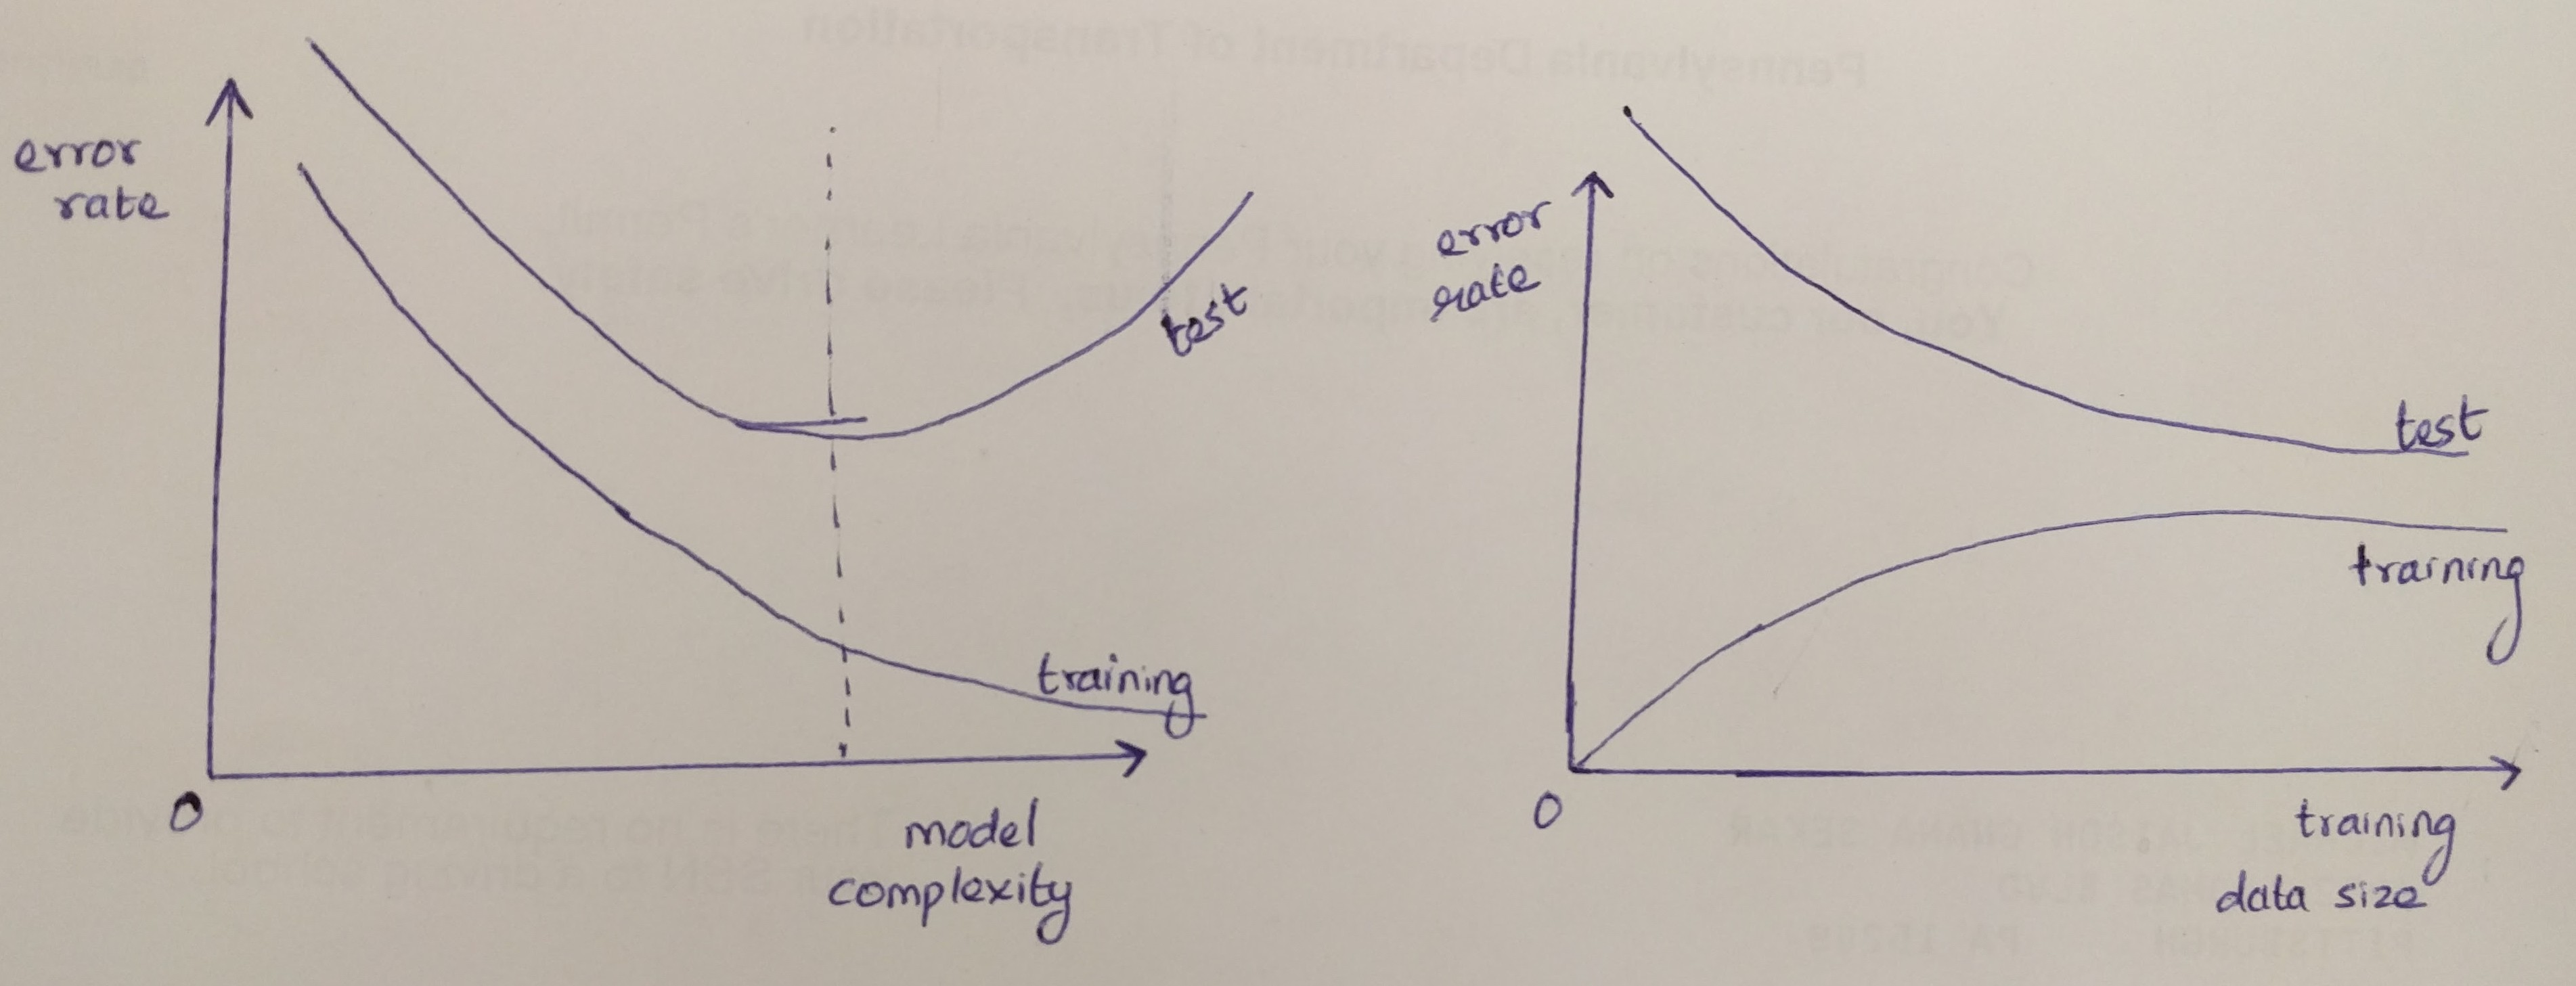
\includegraphics[width=\textwidth]{figures/1}
  \caption{Error rate vs model-complexity and training-size}
  \label{fig:1}
\end{figure}


\section{Problem 2}

\begin{align*}
\mathbf{E}[L_q] = \int \int \mid y(x) - t \mid ^ q p(x, t) dt dx
\end{align*}

The minimum expected loss for q = 1 is given by differentiating and equals to zero.

\begin{align*}
\frac{\partial \mathbf{E}[L_q] }{dx} &= \int sign(y(x) - t)  p(x, t) dt = 0 \\
&= \int_{t < y(x)}  p(x, t) dt + \int_{t >= y(x)} -  p(x, t) dt = 0 \\
\end{align*}

\[
\int_{t < y(x)}  p(x, t) dt = \int_{t >= y(x)} p(x, t) dt
\]

Hence the probability mass for $t < y(x)$ is the same as for $t >= y(x)$.

2.b) As q tends to 0, the loss $(y(x) - t)^q$ becomes approximately 1 and the loss is zero only when $y(x) = t$. This can be visualized as a dip in the graph only when $y(x) = t$. Hence the minimum expected loss is given by the conditional mode.

\section{Problem 3}

A general loss function for a binary classification problem with $t$ as target and $y$ as prediction function, is given by,
$$
E(y) = t . log (y) + (1 - t) log (1 - y)
$$
Since the target $t$ has an error of $\epsilon$, the above loss function cannot be directly used. Instead a penalty of $\epsilon$ should be applied to its prediction.
Substitute $y$ as $y (1 - \epsilon) + (1 - y) \epsilon$

$$
E(y) = t . log (y (1 - \epsilon) + (1 - y) \epsilon) + (1 - t) log (1 - (y (1 - \epsilon) + (1 - y) \epsilon)))
$$

By substituting $\epsilon = 0$, we will get back y.
$$
y (1 - 0) + (1 - y) * 0 = y
$$

\section{Problem 4}

Generalized univariate Gaussian distribution:
$$
p(x|\sigma, q) = \frac{q}{2(2\sigma^2)^{1/q}\Gamma(1/q)} exp \bigg( - \frac{\mid x \mid^q}{2\sigma^2} \bigg)
$$

To show that the distribution is normalized, the integration should sum to 1.

$$
\int_{-\infty}^{\infty} \frac{q}{2(2\sigma^2)^{1/q}\Gamma(1/q)} exp \bigg( - \frac{\mid x \mid^q}{2\sigma^2} \bigg) dx = 1
$$

It is same as proving,
$$
\int_{-\infty}^{\infty} exp \bigg( - \frac{\mid x \mid^q}{2\sigma^2} \bigg) dx = \frac{2(2\sigma^2)^{1/q}\Gamma(1/q)}{q}
$$

Since gaussian is symmetric,
$$
\int_{-\infty}^{\infty} exp \bigg( - \frac{\mid x \mid^q}{2\sigma^2} \bigg) dx = 2 \int_{0}^{\infty} exp \bigg( - \frac{x^q}{2\sigma^2} \bigg) dx
$$

Let $u$ be $\frac{x^q}{2\sigma^2}$

\begin{align*}
u &= \frac{x^q}{2\sigma^2} \\
du &= \frac{qx^{q-1}}{2\sigma^2} dx \\
dx &= \frac{2\sigma^2}{qx^{q-1}} du \\
x &= (2\sigma^2u)^{1/q}  \\
x^{q-1} &= (2\sigma^2u)^{1-1/q}
\end{align*}

Hence, by substituting $u$, we get,

\begin{align*}
2 \int_{0}^{\infty} exp \bigg( - \frac{x^q}{2\sigma^2} \bigg) dx &= 2 \int_{0}^{\infty} exp(- u) \frac{2\sigma^2}{q} (2\sigma^2u)^{1/q - 1}  du \\
&= 2 \frac{2\sigma^2}{q} (2\sigma^2)^{1/q - 1} \int_{0}^{\infty} e^{-u}  u^{1/q - 1}  du \\
&= \frac{2(2\sigma^2)^{1/q}\Gamma(1/q)}{q}
\end{align*}

Hence, the above distribution is normalized.

When $q=2$,

\[
\Gamma(1/2) = \sqrt{\pi}
\]

\[
p(x|\sigma) = \frac{1}{(2\pi\sigma^2)^{1/2}\Gamma(1/q)} exp \bigg(-\frac{\mid x \mid^2}{2\sigma^2} \bigg)
\]

The above equation is Gaussian.

\subsection*{Regression model}

\[
p(t|x, w, \sigma) = \frac{q}{2(2\sigma^2)^{1/q}\Gamma(1/q)} exp \bigg( - \frac{\mid t - y(x,w) - \epsilon \mid^q}{2\sigma^2} \bigg) 
\]
Log likelihood function function over $w$ and $\sigma^2$,
\[
\log p(t|x, w, \sigma) = -\frac{1}{2\sigma^2} \sum_{n=1}^{N} \mid y(x_n, w) - t_n \mid ^ q - \frac{N}{q} \log (2\sigma^2) + const
\]


\section{Problem 5}

\subsection{Basic generalization}

\begin{figure}[!h]
  \centering
  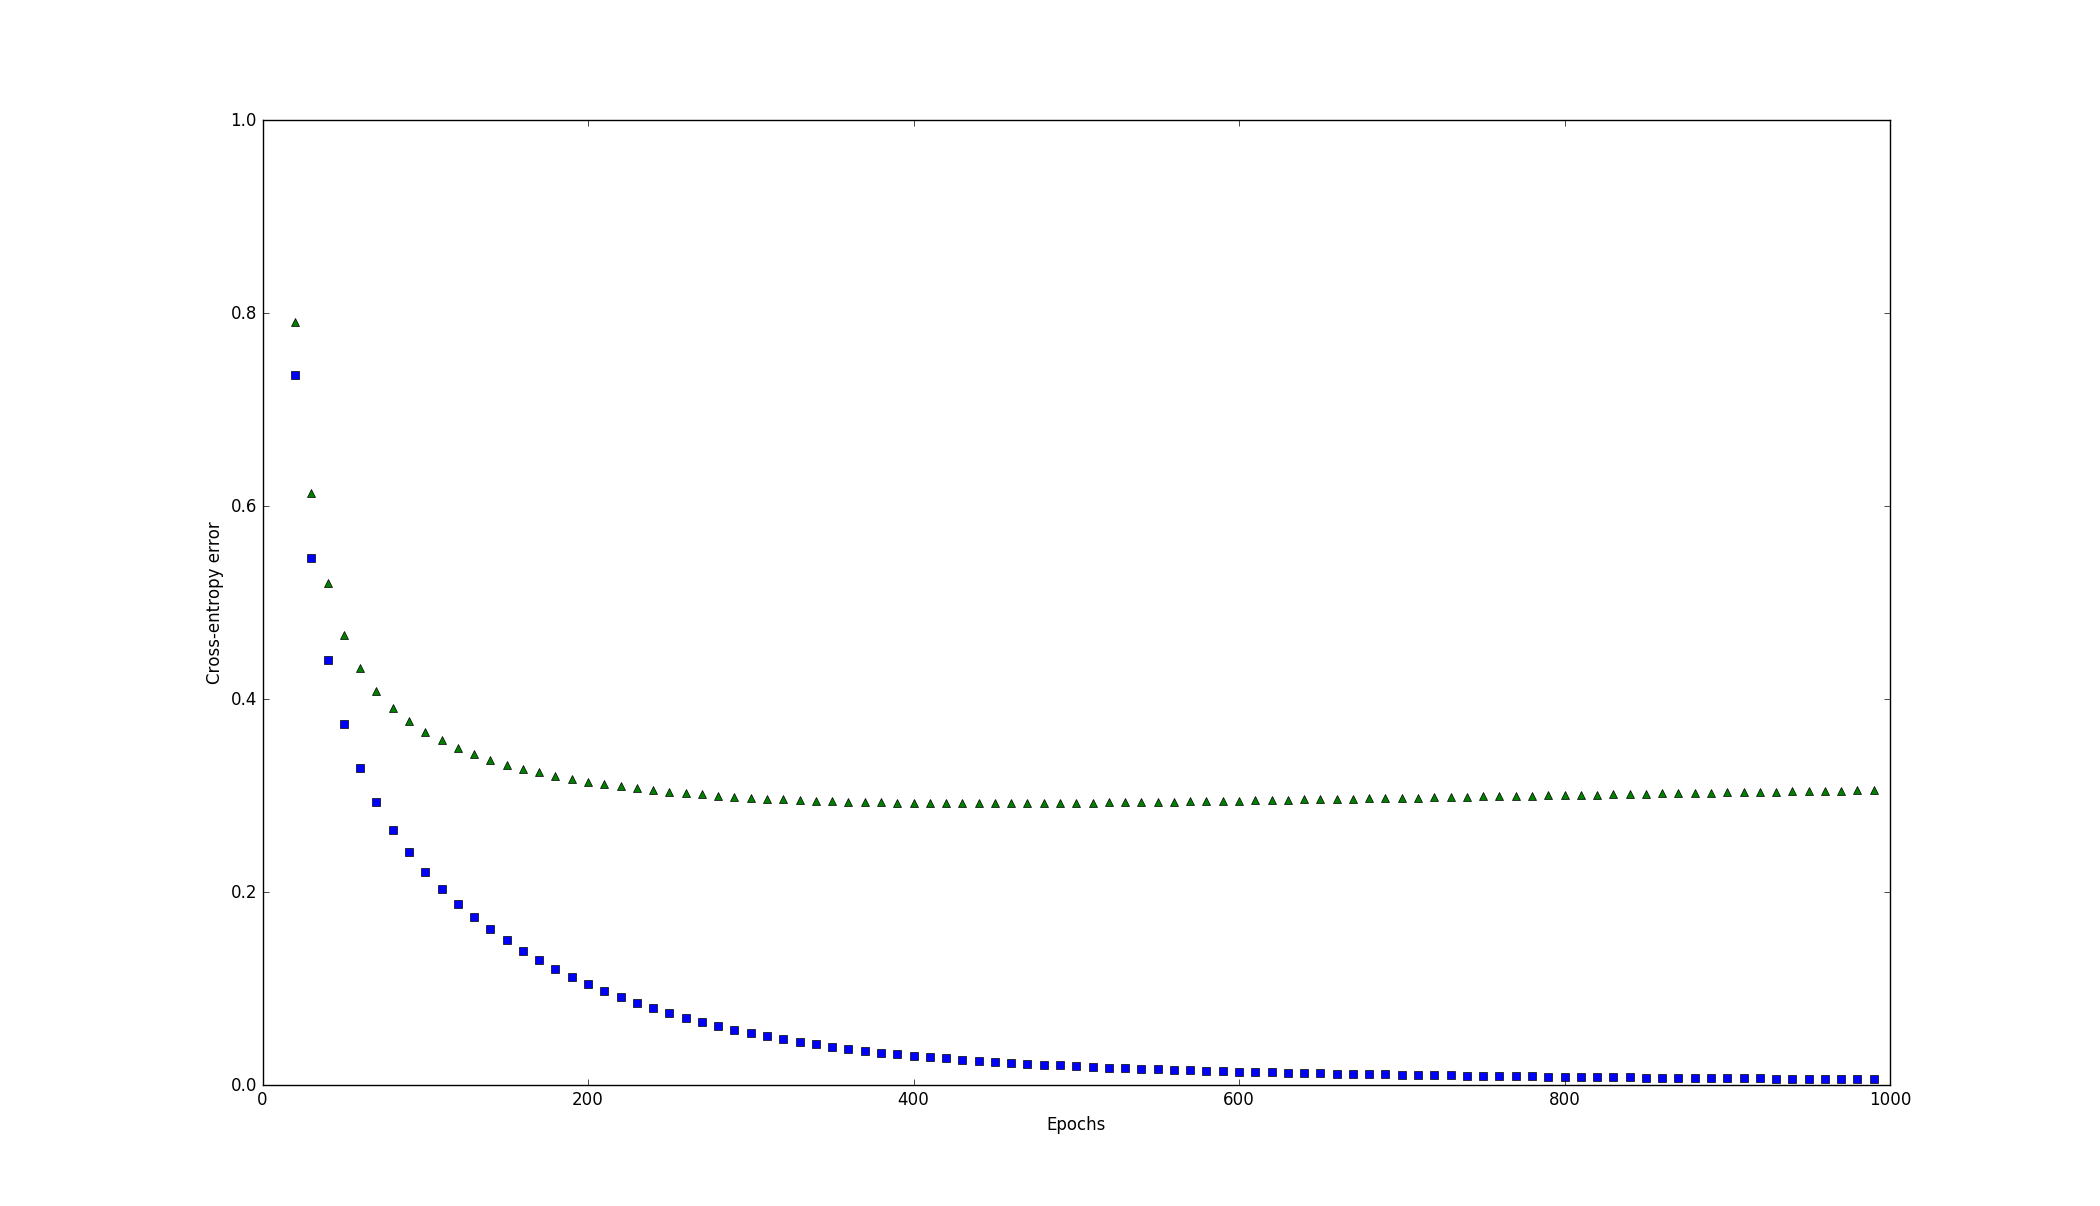
\includegraphics[width=\textwidth]{figures/5a}
  \caption{Cross-entropy error vs epochs.}
  \label{fig:5a}
\end{figure}

The network performance improves continuously for each iteration on the training set. On the other hand, after some number of iterations, the network performance either saturates or lightly decrease for the validation set. This indicates that the network is overfitting for the training data and fails to generalize. Figure \ref{fig:5a} illustrates the performance of the network for both training and validation set.

\subsection{Classification error}

\begin{figure}[!h]
  \centering
  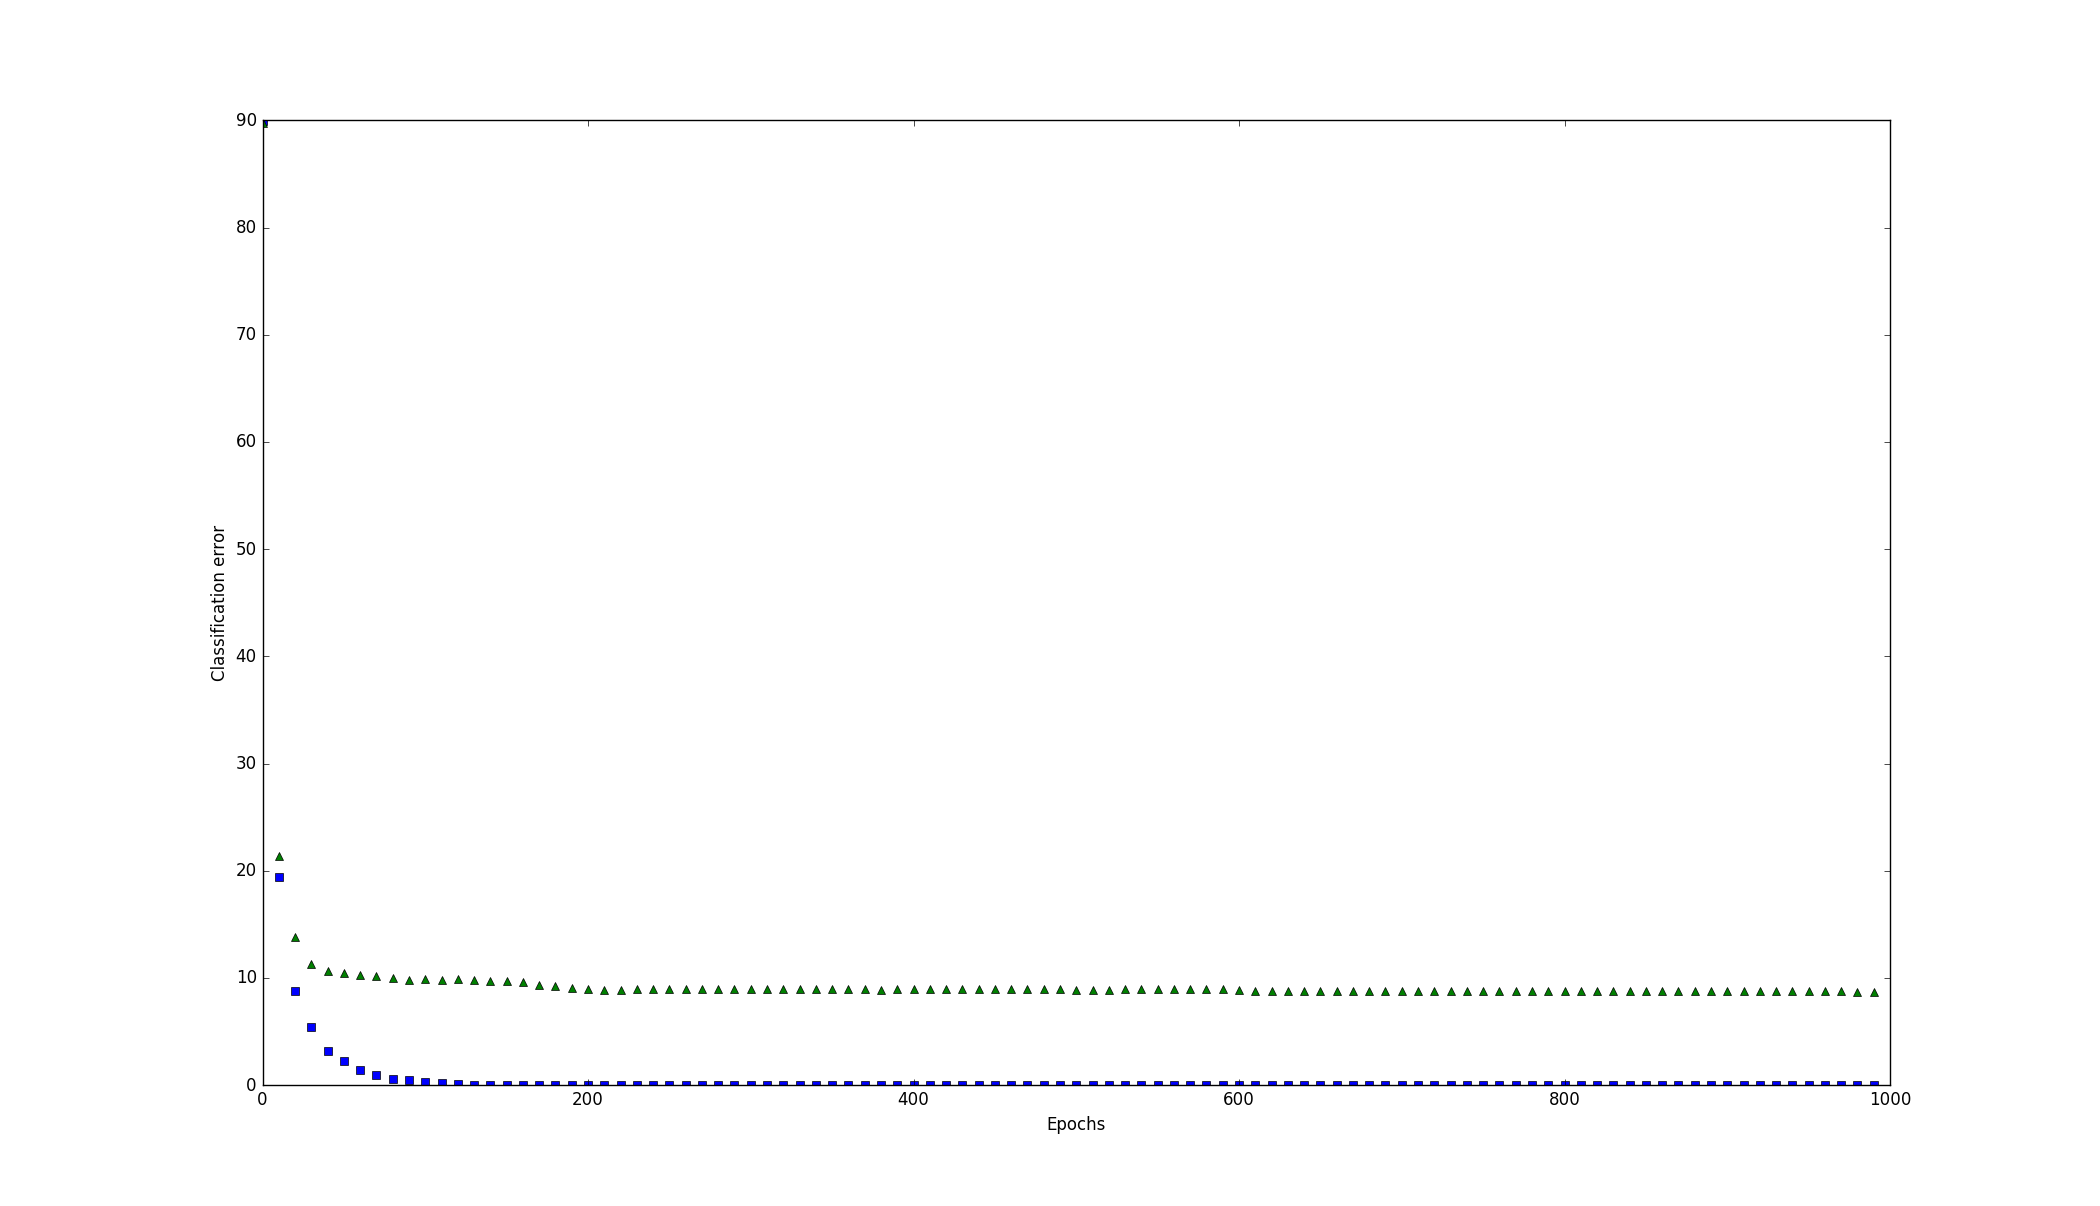
\includegraphics[width=\textwidth]{figures/5b}
  \caption{Classification error vs epochs.}
  \label{fig:5b}
\end{figure}

Classification error is different from the cross-entropy error function. Even though both cross-entropy and classification error are co-related, the network is really trying to optimize the cross-entropy loss rather than the classification error. Also classification error does not provide information about the confidence of the predictions. Hence, the cross-entropy error reduces to zero more earlier than cross-entropy error. Figure \ref{fig:5b} illustrates the performance of the network in terms of classification error.


\subsection{Visualizing parameters}

\begin{figure}[!h]
  \centering
  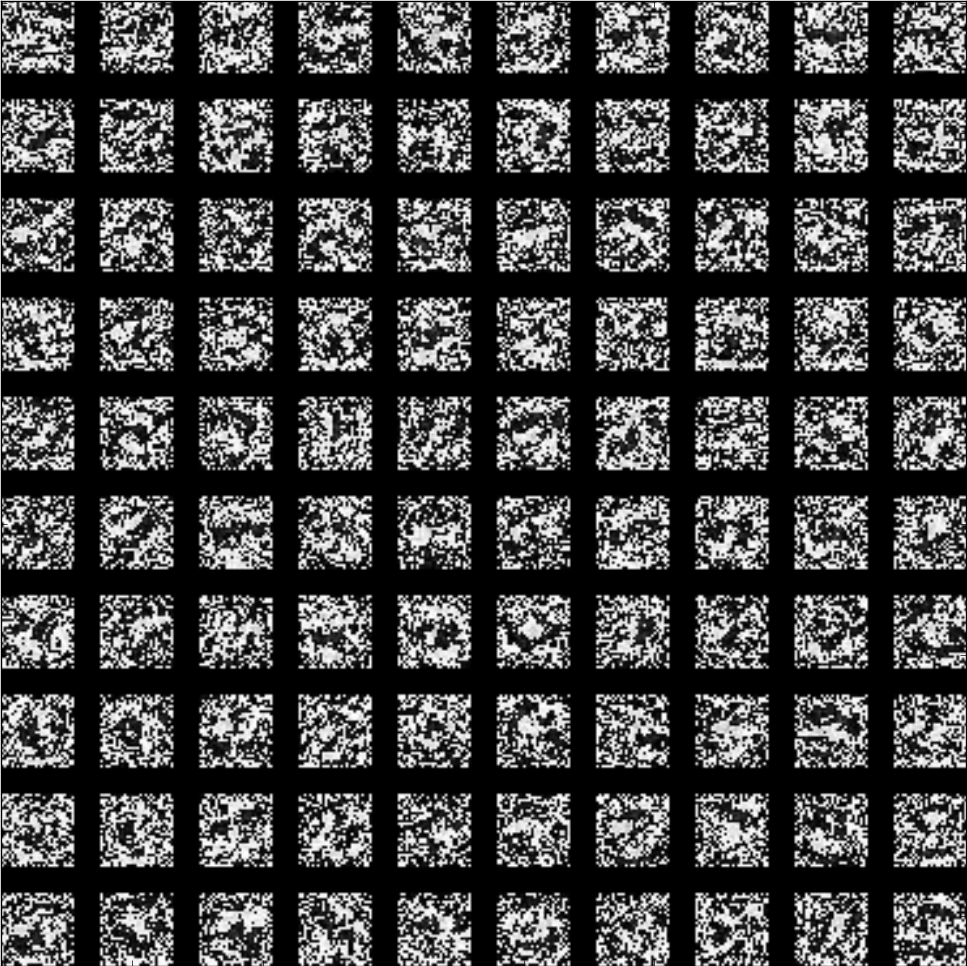
\includegraphics[width=\textwidth]{figures/5c}
  \caption{Visualization of parameters}
  \label{fig:5c}
\end{figure}

By analzying the visualization of the network parameters, it looks like the digit characters are hidden inside the weights. For example, the weights in 5th row, 2nd column looks like an inverted digit '5'. Similarly 5th row, 3rd column looks like a digit '3'. It seems like that the each neuron is trying to extract features that can help classify the image in one of the ten classes. Since it is a single layer network, the network did not learn any hierarchy of features.

\subsection{Learning rate and Momentum}

\subsubsection*{Learning rate}
In Figure \ref{fig:5d1}, It can be noticed that with learning-rate = 0.01, the error values decrease consistently and slowly. Even after 1000 epochs, the network did not overfit the training data. This will help the network to avoid outliers if present in the training data. On the otherhand, learning-rate as 0.2 or 0.5, makes the network converge early. But higher learning-rate, also overfits to the training data quickly when compared to lower values. The difference can be easily visualized at epoch 200.

\subsubsection*{Momentum}
All the other hyper parameters are fixed, and momentum is experimented for different values: 0, 0.5, and 0.9. From the experiment, it is noticed that higher momentum helps to converge very early. It only takes a very few epochs to reduce the training cross-entropy error. In Figure \ref{fig:5d2}, it can be noticed that as momentum increases, the training cross-entropy error reduces  early. The difference in error can be easily noticed at epoch 200. But when momentum is increased to 0.9, the validation error is huge comparitively. \\

The best values of these parameters can be chosen based on the convergance property. The value should be chosen when the network performs well on both training and validation set. If the data has a lot of outliers, choosing lower learning rate might reduce the effect of those outliers passing to the learned weights. \\

The best value of momentum can be chosen by noticing the progress of convergence. If the convergence is really slow, adding a little momentum will help smooth out the inconsistent gradients.

\begin{figure}[!h]
  \centering
  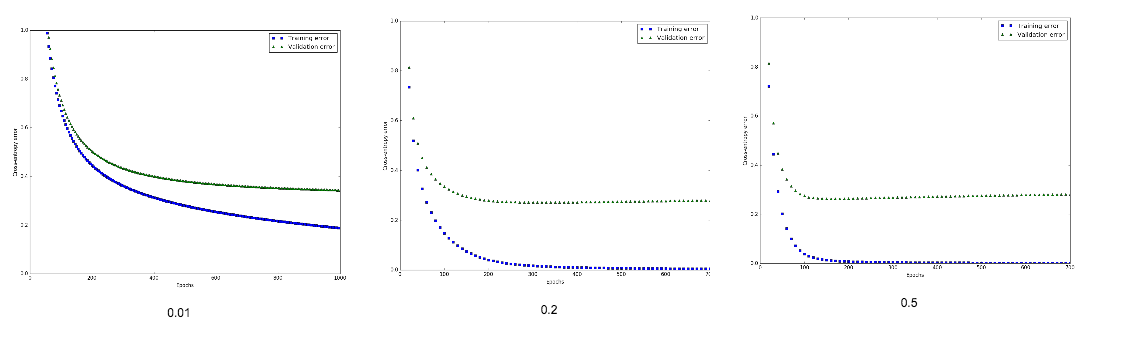
\includegraphics[width=\textwidth]{figures/5d1}
  \caption{Effect of Learning rate}
  \label{fig:5d1}
\end{figure}

\begin{figure}[!h]
  \centering
  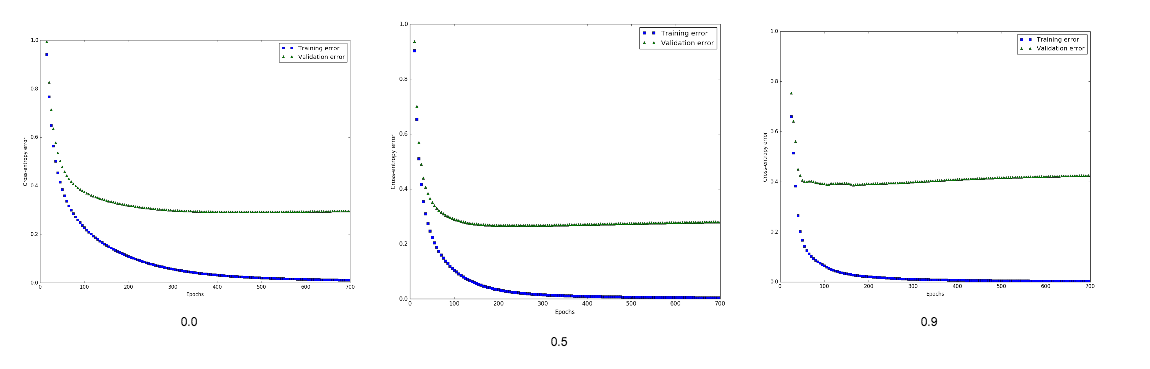
\includegraphics[width=\textwidth]{figures/5d2}
  \caption{Effect of momentum}
  \label{fig:5d2}
\end{figure}


\subsection{Number of hidden units}

From Figure \ref{fig:5e}, It can be noticed that adding more neurons did not show much difference in terms of convergence or generalization of the network. It can be inferred that most of the neurons might be learning same information about the images. In case of 500 neurons, most neurons might firing for the same featu

\begin{figure}[!h]
  \centering
  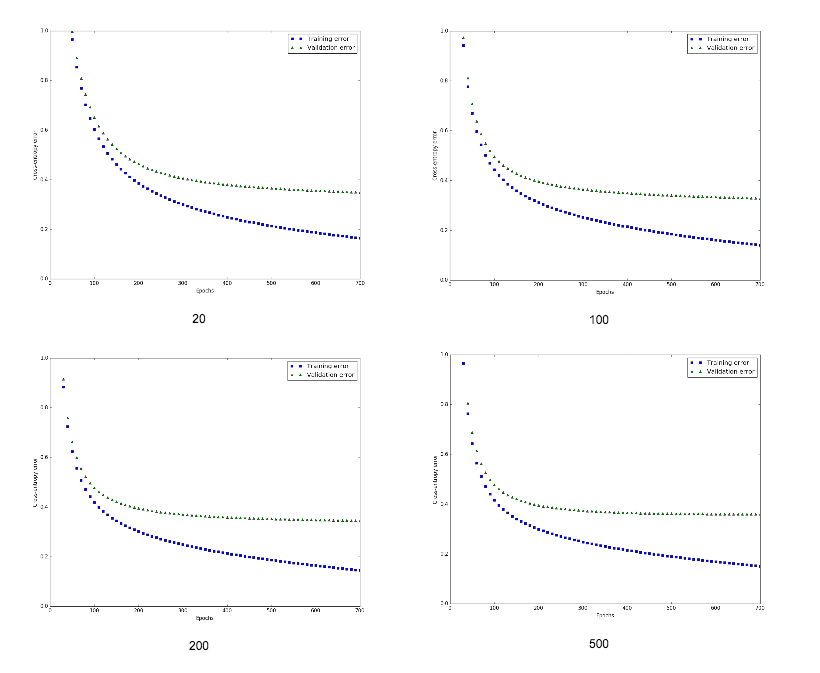
\includegraphics[width=\textwidth]{figures/5e}
  \caption{Effect of number of hidden units}
  \label{fig:5e}
\end{figure}


\subsection{Dropout}
Dropout helped the network to generalize but the training error decreased little slowly when compared with zero dropout. Figure \ref{fig:5f} shows the effect of dropout = 0.5 on convergence and generalization. The classification error is less for validation set when dropout is used, which explains the network generalization.


\begin{figure}[!h]
  \centering
  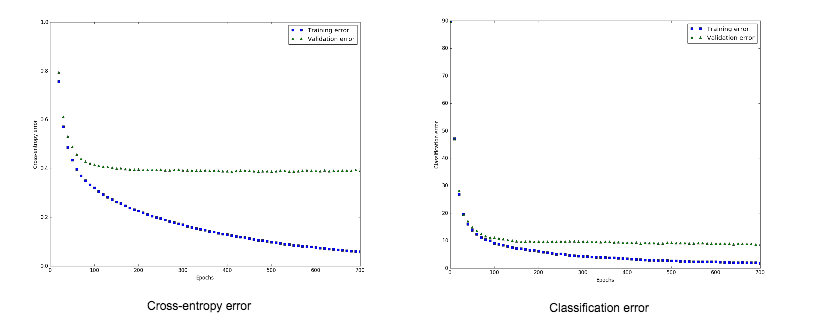
\includegraphics[width=\textwidth]{figures/5f}
  \caption{Effect of dropout = 0.5}
  \label{fig:5f}
\end{figure}


\subsection{Best performing single-layer network}

Apart from the hyper parameter provided in the homework, I have added data normalization as an initial step before training and testing. It looks like normalization helps the network to converge very quickly. In the experiments, it is noticed that with normalization the network converged at 340 epochs while without normalization the network converged at 520 epochs.

Also all the experiments are implemented with Stocastic gradient descent with mini-batch size 100. In another experiment it is noticed that shuffling these mini-batch boosts the convergence time too. With shuffling, the network converged at 290 epochs compared to 340 epochs. All other experiments were run with normalization and shuffling.

I got best validation performance for \\
Number of hidden units: 100 \\ 
learning-rate: 0.1 \\ 
momentum: 0.5 \\ 
dropout: 0.3 \\ 
weight-decay: 0.005 \\
Early epoch stop: 250 \\

The final perfomance of the network on Test data is mentioned below. \\

Average Cross entropy (Training): 0.04 \\
Average Classification error (Training): 0.3\% \\

Average Cross entropy (Validation): 0.306 \\
Average Classification error (Validation): 8.7\% \\

Average Cross entropy (Test): 0.384 \\
Average Classification error (Test): 9.06\% \\

The weights visualization can be seen in Figure \ref{fig:5g}

\begin{figure}[!h]
  \centering
  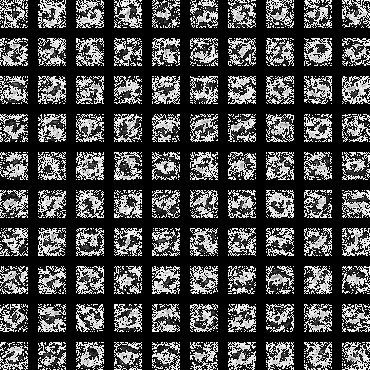
\includegraphics[width=\textwidth]{figures/5g}
  \caption{Visualization of one-layer network weights}
  \label{fig:5g}
\end{figure}


\subsection{Extension to multiple layers}

It is found that adding an extra layer did not show much improvement on the test performance. It might be because that the dataset does not have much variance to learn. We have also observed that the number of neurons in the first layer did not show up great impact. The two-layer architecture seems to be more robust to over-fitting with the same number of epochs. One reason is because the power of gradients is reduced as it traverses back each layer.

I got best validation performance for \\
Number of hidden units: [100, 40] \\ 
learning-rate: 0.1 \\ 
momentum: 0.5 \\ 
dropout: 0.3 \\ 
weight-decay: 0 \\
Early epoch stop: 500 \\

The final perfomance of the network on Test data is mentioned below. \\

Average Cross entropy (Training): 0.027 \\
Average Classification error (Training): 0.533\% \\

Average Cross entropy (Validation): 0.383 \\
Average Classification error (Validation): 7.6\% \\

Average Cross entropy (Test): 0.501 \\
Average Classification error (Test): 9.63\% \\

The weights visualization can be seen in Figure \ref{fig:5h}. Even though, there are not much difference in the learned weights, It seems like these weights have learned a better understanding of images. Interesting patterns can be seen in the Figure.

Layer-1 network and Layer-2 network performs very similar to each other. In terms of generalization, Layer-2 networks seems reasonable.

\begin{figure}[!h]
  \centering
  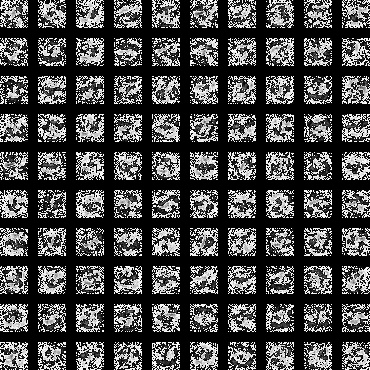
\includegraphics[width=\textwidth]{figures/5h}
  \caption{Visualization of two-layer network weights}
  \label{fig:5h}
\end{figure}




\end{document}
